\chapter{Scalable Rendering Process}\label{chapter_scalable_rendering_process}



Rendering the planet file from zoom level 0 to zoom level 14 requires $\sum_{i=1}^{14} 4^i = 357\,913\,941$ tiles to be rendered. 
Rendering this amount of tiles serially is no longer possible due to two problems.

\begin{itemize}
    \item The rendering process might fail and progress is lost
    \item A single worker process takes approximately 276 days to render the planet with a throughput of $54\,000$ tiles per hour
\end{itemize}

To solve these problems two measurements described in \autoref{split-rendering-process-task} and \autoref{list-job} have been taken.

%-----------------------------------------
\section{Split Rendering Process into Jobs}\label{split-rendering-process-task}

The rendering process (Mapnik)
renders tiles within the given bounding box into a SQLite database (MBTiles). To adapt the process the global bounding box needs to be divided into many smaller bounding boxes and the many small SQLite databases need to be merged together into a large planet SQLite database at the end of the process.
The unit of a job therefore is a bounding box derived from a XYZ tile index (pyramid job \autoref{pyramid-job}) or a list of tiles (list job \autoref{list-job}).

\begin{figure}[H]
  \centering
  \includegraphics[width=0.9\textwidth]{images/split_and_merge_sqlite.png}
  \caption{Adapt rendering process to divide work and merge it back together}
\end{figure}

\subsection{Pyramid Job}\label{pyramid-job}

To divide the work for rendering the planet into equal parts across the world the XYZ coordinate schema described in \autoref{part1_xyz_coordinates} is used to divide the planet into several subpyramids.

\subsubsection*{Algorithm}

\begin{enumerate}  
    \item Choose job zoom level $z$ and maximum zoom level $Z$
    \item Calculate the $4^z$ tiles for job zoom level
    \item Convert XYZ tile index into a WGS84 bounding box
    \item Render bounding box from zoom level $z$ down to the maximum zoom level $Z$
\end{enumerate}

\begin{figure}[H]
  \centering
  \includegraphics[width=0.8\textwidth]{images/pyramid_job.png}
  \caption{Pyramid job of a zoom level 2 tile and the descendants}
\end{figure}

\subsubsection*{Example}

Given the job zoom level $z=8$ and the max zoom level $Z=14$ the planet is divided into $4^{8}$ jobs.
This means each subpyramid task consists of rendering all descendant tiles from a tile at zoom level 8.
Each job therefore consists of $\sum_{i=0}^{6} 4^i = 5\,461$ tiles that need to be rendered.  \\

\begin{figure}[H]
  \centering
  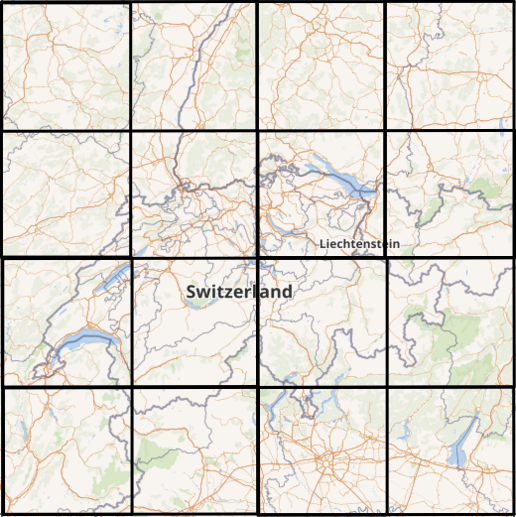
\includegraphics[width=0.4\textwidth]{images/switzerland_tiled_z8_small.png}
  \caption{Map divided into tasks at job zoom level 8}
\end{figure}

%-----------------------------------------
\section{List Job}\label{list-job}

It is important to be able to update distinct tiles to fix bugs later on or rerender all changed geometries. A list job is a batch job of tiles grouped together by their proximity and is created from a large list of tiles. The primary use case is to process the large list of changed tiles that need to be rerendered each week ($20\,000\,000$ to $30\,000\,000$ tiles).

\subsubsection*{Algorithm}

To group tiles that are in close proximity in one batch job the tiles are sorted lexically by their Quadkey.

\begin{enumerate}  
    \item Given a large list of tiles
    \item Calculate Quadkey of XYZ tile index
    \item Sort lexically by Quadkey
    \item Split list into sublists of batch size
\end{enumerate}

\subsubsection*{Quadkey}

The Quadkey has several unique properties which makes it ideal for grouping
tiles together.

\begin{enumerate}  
    \item Length indicates level of detail
    \item Quadkey starts with Quadkey of parent tile
\end{enumerate}

\begin{figure}[H]
  \centering
  \includegraphics[width=0.65\textwidth]{images/quadkey.png}
  \caption{Quadkey indexing}
\end{figure}

\subsubsection*{Implementation}

The Python implementation of the algorithm is straightforward and consists of
calculating the Quadkey from a XYZ, sorting by it and splitting it into
sublists of the desired batch size.

\begin{pythoncode}
tiles = [Tile(0, 0, 0), Tile(0, 1, 0), ..]
tiles.sort(key=lambda t: quad_tree(t.x, t.y, t.z))
batch_jobs = split_tiles_into_batch_jobs(tiles, batch_size=1000)

def quad_tree(tx, ty, tz):
    quad_key = ''
    for i in range(tz, 0, -1):
        digit = 0
        mask = 1 << (i-1)
        if (tx & mask) != 0:
            digit += 1
        if (ty & mask) != 0:
            digit += 2
        quad_key  += str(digit)

    return quad_key
    
def split_tiles_into_batch_jobs(tiles, batch_size):
    tiles_batch = []
    
    for tile in tiles:
        tiles_batch.append(tile)
        if len(tiles_batch) > batch_size:
            yield tiles_batch
            tiles_batch = []

    yield tiles_batch
\end{pythoncode}

%--------------------------------------
\newpage
\section{Distributed Architecture}

To distribute across several hosts a distributed architecture (\autoref{distributed_rendering_architecture}) using job queues has been implemented.

\begin{enumerate}  
    \item Pyramid or list jobs are created by \texttt{generate-jobs} and put into the \texttt{jobs} queue
    \item The different worker processes on different hosts poll the \textbf{jobs} queue for new jobs and try to render them in the given time frame.
    \item If the rendering does not complete in the given time frame it is put into the \texttt{failed-jobs} queue.
    \item The resulting SQLite database is uploaded to a S3 compatible object store and linked in the result message which is stored in the \textbf{results} queue.
\end{enumerate}


\begin{figure}[H]
  \centering
  \includegraphics[width=0.9\textwidth]{images/distributed_rendering_architecture.png}
  \caption{Distributed rendering architecture using message queues}
  \label{distributed_rendering_architecture}
\end{figure}

\subsubsection{Dealing with Errors}

The message queue is using an acknowledge mechanism together with durable queues.
This means if any process fails at any stage in the workflow (\textbf{render} or \textbf{merge}) the message is requeued and redelivered to the next worker.
Since there are always some jobs that never complete or have very distinct problems the timeout prevents the workers from being jammed by the same failing jobs over and over again.
Failed jobs can be inspected and rescheduled at a later point in time.

\newpage{}
%----------------------------
\section{Merging Results}

A very important part of the workflow is merging all of the $65\,536$ SQLite databases.
The \texttt{merge-jobs} process downloads the linked SQLite database in the result message
and then merges it into the specified merge target (e.g. the Planet MBTiles file).

\begin{enumerate}  
    \item Message is consumed from the \texttt{results} queue.
    \item The linked SQLite database is downloaded from S3.
    \item The downloaded SQLite database is attached to the merge target.
    \item  The data tables \texttt{map} containing the tile indizes and \texttt{images} containing the actual PBF data are copied over replacing the already existing entries in the database.
    
\begin{sqlcode}
ATTACH DATABASE 'source.mbtiles' AS source;
REPLACE INTO map SELECT * FROM source.map;
REPLACE INTO images SELECT * FROM source.images;
\end{sqlcode}
    
\end{enumerate}

\begin{figure}[H]
  \centering
  \includegraphics[width=0.88\textwidth]{images/merge-jobs.png}
  \caption{Merge completed MBTiles files together}
\end{figure}

This is a very fast way of distributing updates to an MBTiles file which can be applied with any SQLite client and performs for many small databases merged into one large merge target.

\newpage{}
%----------------------------
\section{Save Space by removing identical subpyramids}

Water tiles is a large part of the resulting planet file since most of the earth is covered in water.
If a tile only contains water it is not desirable to store the same water geometry on all zoom levels
from z8 down to z14 (resulting in $\sum_{i=0}^{6} 4^i = 5\,461$ tiles all containing the same geometry).
To prevent this issue all z8 subpyramids containg the same data on all descendant tiles are removed.

\subsubsection*{Algorithm}

\begin{enumerate}  
    \item Calculate all descendant tiles of a given parent tile
    \item Calculate SHA1 checksum for each tile
    \item Count occurences of each unique checksum
    \item Ensure there is only one checksum used in all descendants
    \item If checksum matches parent tile checksum remove all descendants
\end{enumerate}


\begin{figure}[H]
  \centering
  \includegraphics[width=0.6\textwidth]{images/remove_identical_subtiles.png}
  \caption{A z8 subpyramid with the same data hash in all descendant tiles}
\end{figure}
